\documentclass[11pt]{beamer}

\usepackage[czech]{babel}
\usepackage[czech]{algorithm2e}
\usepackage{pict2e}

\usetheme{Boadilla}

\title{Typografie a publikování -- 5. projekt}
\subtitle{Breadth-First Search Algorithm}
\author{Denys Petrovskyi}
\date{\today}

\begin{document}

\begin{frame}
    \maketitle
\end{frame}

\begin{frame}
    \frametitle{Úvod}
    \begin{itemize}
        \item Co je BFS a jak se používá?
        \item Jaké jsou výhody BFS?
        \item Příklady
    \end{itemize}
\end{frame}

\begin{frame}
    \frametitle{Definice BFS}
    \begin{itemize}
        \item BFS je algoritmus procházení, 
        který začíná v kořenovém uzlu a zkoumá všechny uzly v aktuální hloubce, 
        než se přesune k uzlům v další hloubce.
        \item BFS navštíví všechny uzly v grafu, ale pořadí, ve 
        kterém jsou uzly navštíveny, závisí na struktuře grafu.
        \item BFS lze použít k nalezení nejkratší cesty mezi dvěma uzly v neváženém grafu.
    \end{itemize}
\end{frame}

\begin{frame}
    \frametitle{Složitost algoritmu}
    \textbf{Časovou složitost} lze vyjádřit jako $O ( | V | + | E | )$,
    protože v nejhorším případě bude prozkoumán každý vrchol a každá hrana.
    \begin{itemize}
        \item $|V|$ je počet vrcholů v grafu
        \item $|E|$ je počet hran v grafu
    \end{itemize}
    \textbf{Prostorová složitost} je $O(B^M)$, kde:
    \begin{itemize}
        \item $B$ je nejvyšší stupeň větvení stromu
        \item $M$ je nejvyšší délka cesty ve stromě
    \end{itemize}
\end{frame}

\begin{frame}
    \frametitle{Pseudokód}
    \begin{algorithm}[H]
        \SetKwInOut{Input}{Input}\SetKwInOut{Output}{Output}
        \Input{Graf $G$ a počáteční uzel $s$}
        \Output{Nejkratší cesta z $s$ do všech ostatních uzlů v $G$}
        \BlankLine
        \For{$u \in U(G) - {s}$}{
            $stav[u] = FRESH$; $d[u] = \infty$; $p[u] = null$;
        }
        $stav[s] = OPEN$; $d[s] = 0$; $p[s] = null$; $Queue.Init()$; $Queue.Push(s)$;
        \While{$!Queue.Empty()$}{
            $u = Queue.Pop()$;\\
            \For{$v \in Adj[u]$}{
                \If{$stav[v] == FRESH$}{
                    $stav[v] = OPEN$; $d[v] = d[u]+1$; $p[v] = u$; $Queue.Push(v)$;
                }
            }
        $stav[u] = CLOSED$;
        }
        \end{algorithm}
\end{frame}

\begin{frame}
    \frametitle{Obrázky}
    \begin{figure}[ht]
        \begin{center}
            \scalebox{0.15}{\includegraphics{BFST.eps}}
            \caption{Příklad BFS}
        \end{center}
    \end{figure}
\end{frame}

\begin{frame}
    \frametitle{Obrázky}
    \begin{figure}[ht]
        \begin{center}
            \scalebox{0.5}{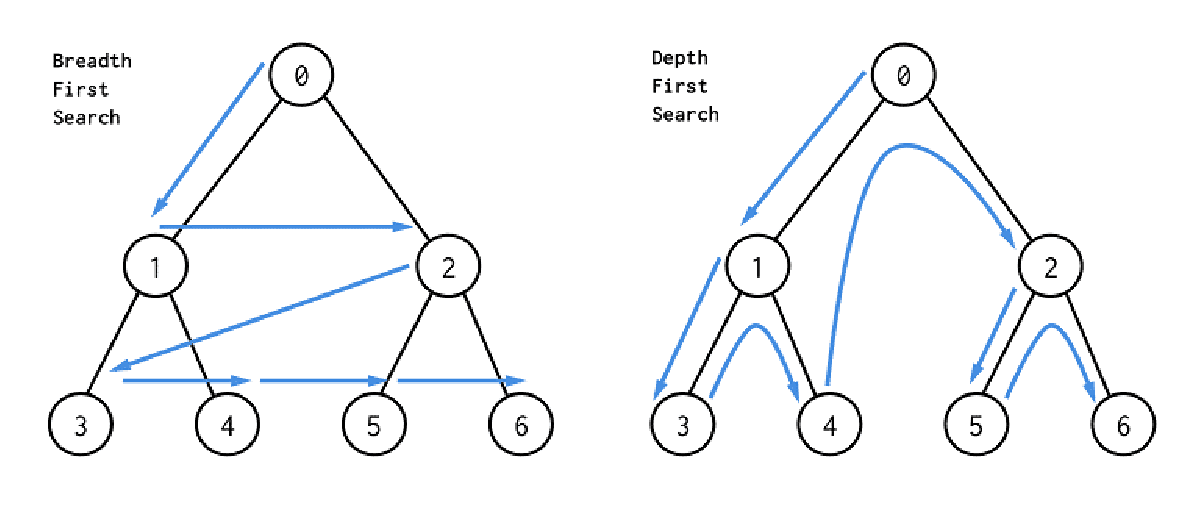
\includegraphics{BFS-and-DFS-Algorithms.eps}}
            \caption{Srovnání BFS a DFS}
        \end{center}
    \end{figure}
\end{frame}

\begin{frame}
    \frametitle{Závěr}
    \begin{itemize}
        \item BFS je základní grafový algoritmus, který se používá v mnoha aplikacích
        \item Má časovou složitost $O(|V|+|E|)$ a prostorovou složitost $O(B^M)$
        \item BFS lze použít k nalezení nejkratší cesty mezi dvěma vrcholy, kontrole, zda je graf propojen, a zjištění průměru grafu
    \end{itemize}
\end{frame}
    
\end{document}